\section{Background}                     % context and prior work the project builds on
\label{sec:background}                   % \secref{sec:background}

This project continues a previous internship on the 3D reconstruction of a flooded karst conduit
from sonar data \citep{margaritis2025internship}. This section recalls the scientific context,
how the data were collected, how the existing point cloud was produced from them, and which part
of the data that work left unused.

% ------------------------------------------------------------------------------
\subsection{Karst conduits and the RKE project}   % why these environments are studied
\label{sec:bg_context}                            % \secref{sec:bg_context}

Karst systems form when water dissolves soluble rock such as limestone, creating networks of
underground caves and conduits \citep{ford2007karst}. They store the groundwater used by about a
quarter of the world's population \citep{goldscheider2020karst}. They are also a hazard: water
moves through the conduits quickly and with little filtering, so pollution spreads fast, and
heavy rain can overwhelm the network and cause sudden floods. The Fontaine de N\^imes, the site
studied here, feeds the flash floods that threaten the city; the flood of 3~October~1988 killed
nine people \citep{marechal2008nimes, batiot2013nimes}. Modelling and managing such an aquifer
requires knowing the geometry of its conduits, yet many of them are out of reach for human divers.
The \emph{Robots for Karst Exploration} (RKE) project therefore develops robotic platforms to map
these flooded networks \citep{lapierre2021karst}.

% ------------------------------------------------------------------------------
\subsection{Data acquisition}            % the platform and its sensors
\label{sec:bg_acquisition}               % \secref{sec:bg_acquisition}

The data were recorded in March~2023 in the flooded conduit of the Fontaine de N\^imes with the
NavScoot~2, a diver-propelled vehicle carrying the sensor suite first deployed on the Ulysse robot
\citep{lasbouygues2017karst} (Figure~\ref{fig:bg_navscoot}). Its sensors fall into two groups:
\begin{itemize}                          % sensors grouped by role
  \item \textbf{Navigation:} a Doppler velocity log (DVL, Nortek DVL~1000) for the velocity, an
        inertial measurement unit (IMU, SBG Ellipse~A) for the orientation, a pressure depth
        sensor (Blue Robotics Bar30) and a forward-looking echosounder (ISA~500) with its own
        attitude unit.
  \item \textbf{Mapping:} two mechanically scanned imaging sonars (MSIS). A \emph{vertical}
        profiling sonar (Tritech Super SeaKing, beam width 1--2$^\circ$) sweeps a plane across
        the conduit, measuring its section: roof, floor and walls. A \emph{horizontal} scanning
        sonar (Blue Robotics Ping360) sweeps a full circle in the horizontal plane, with a beam
        2$^\circ$ wide horizontally but 25$^\circ$ high vertically.
\end{itemize}
An MSIS emits one narrow acoustic ping at a time and rotates its head step by step; each ping
returns an intensity profile along a single direction (the \emph{echo}). A full scan is therefore
built over several seconds while the vehicle keeps moving.

\begin{figure}[!htbp]                    % the acquisition platform
  \centering
  \begin{minipage}[b]{0.48\linewidth}    % left: the vehicle
    \centering
    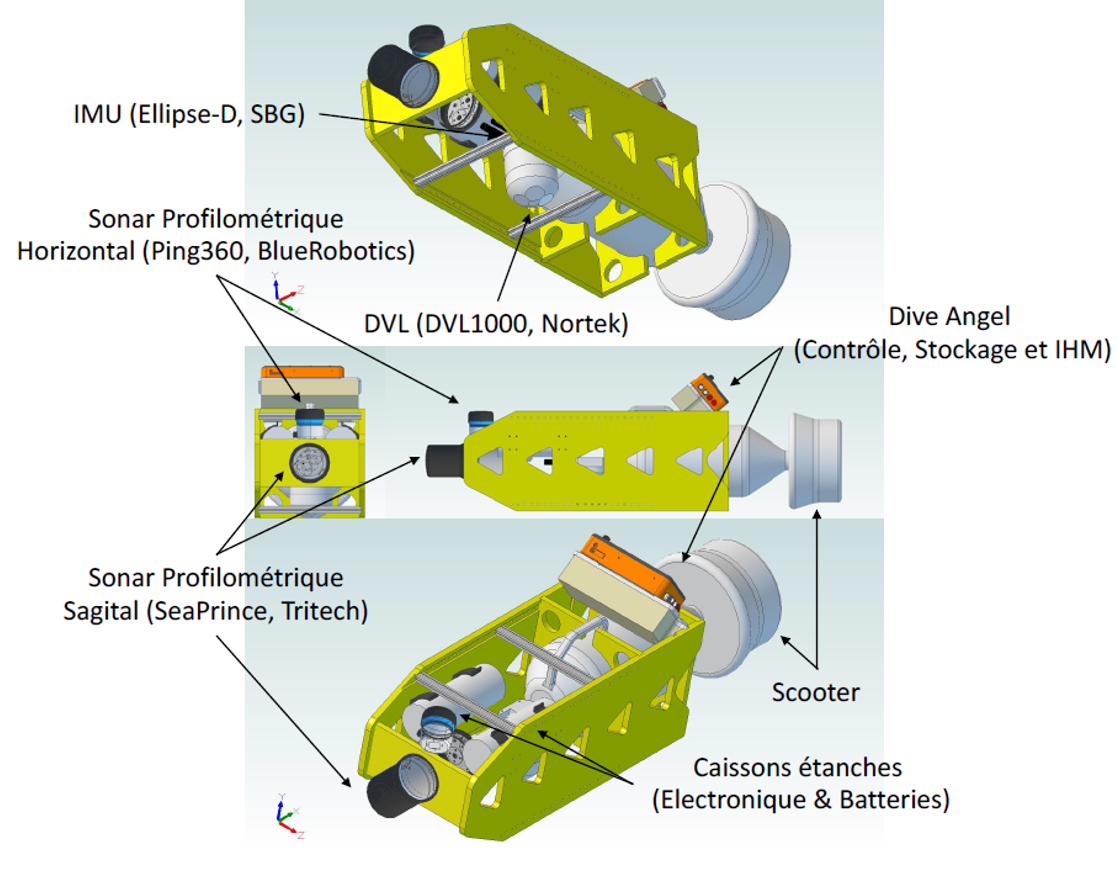
\includegraphics[width=\linewidth, height=5cm, keepaspectratio]{figures/Scooter.png}\\[0.3em]
    {\small (a)}
  \end{minipage}\hfill
  \begin{minipage}[b]{0.48\linewidth}    % right: the diver operating it
    \centering
    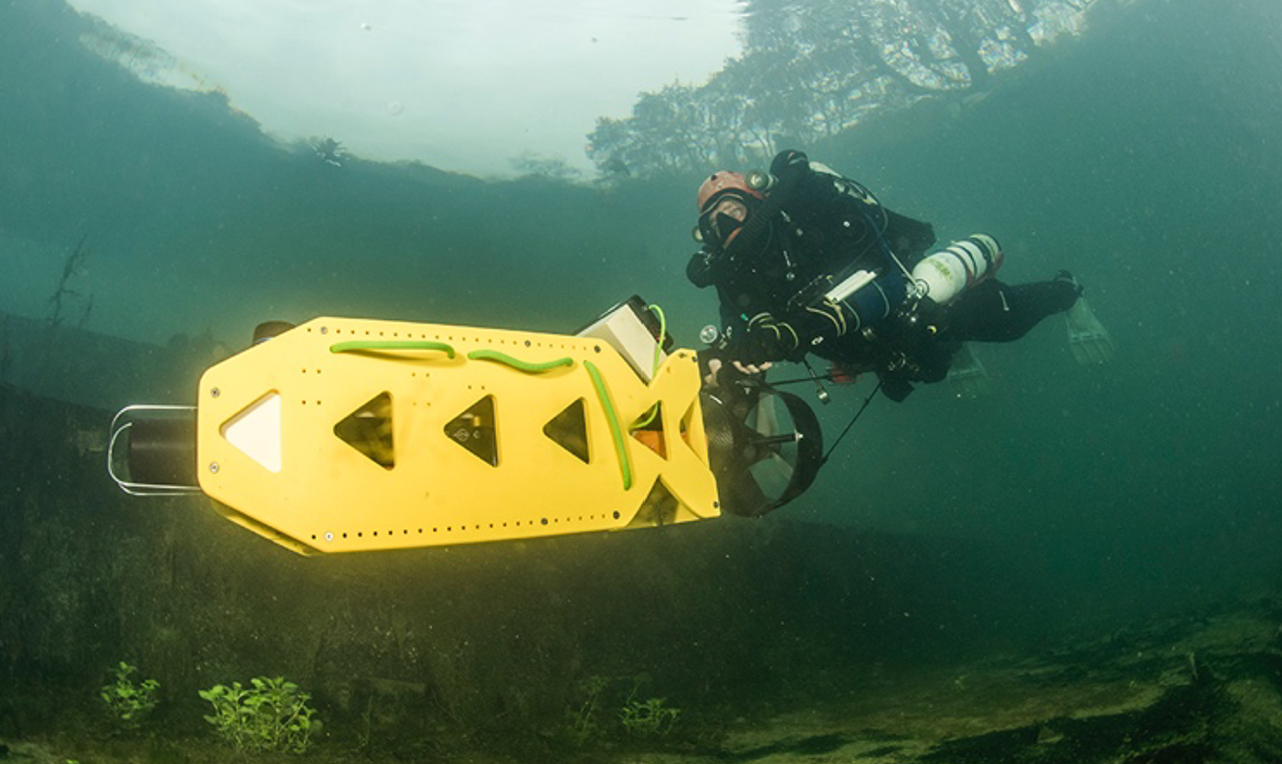
\includegraphics[width=\linewidth, height=5cm, keepaspectratio]{figures/Scooter_diver.png}\\[0.3em]
    {\small (b)}
  \end{minipage}
  \caption{The NavScoot~2 acquisition platform \citep{margaritis2025internship}: (a) the vehicle
           with its sensors; (b) the diver operating it.}
  \label{fig:bg_navscoot}
\end{figure}

% ------------------------------------------------------------------------------
\subsection{From raw data to a point cloud}  % the existing pipeline
\label{sec:bg_pipeline}                      % \secref{sec:bg_pipeline}

The previous work re-implemented the original MATLAB processing chain in Python and corrected
several errors in it \citep{margaritis2025internship}. The pipeline works in three stages:
\begin{enumerate}                        % pipeline stages in order
  \item \textbf{Trajectory.} DVL velocity spikes above 2~m/s are removed, all sensors are
        restricted to their common time window and expressed in the vehicle body frame. The
        velocity is rotated into the world frame with the IMU orientation and integrated over
        time, while the depth sensor gives the vertical position (dead reckoning).
  \item \textbf{Echo detection.} In every ping of the vertical sonar, the noise close to the
        transducer is cut, and the first return above an intensity threshold is kept as the
        distance to the conduit wall; later returns are discarded as multipath echoes.
  \item \textbf{Projection.} Each detection (range, beam angle, time) is placed in 3D using the
        vehicle pose interpolated at the time of the ping, giving a point cloud of about
        50\,000 points.
\end{enumerate}
Integrating velocities accumulates drift, which distorts the point cloud. It was reduced with the
Continuous-time SLAM of the 3D Toolkit (3DTK) \citep{borrmann2008globally, nuchter2017cartographer},
which splits the trajectory into overlapping segments and deforms it smoothly so that the parts
of the cloud that see the same walls align (Figure~\ref{fig:bg_pointcloud}). The corrected cloud
was then turned into a surface mesh with learning-based reconstruction methods.

\begin{figure}[!htbp]                    % the data this project starts from
  \centering
  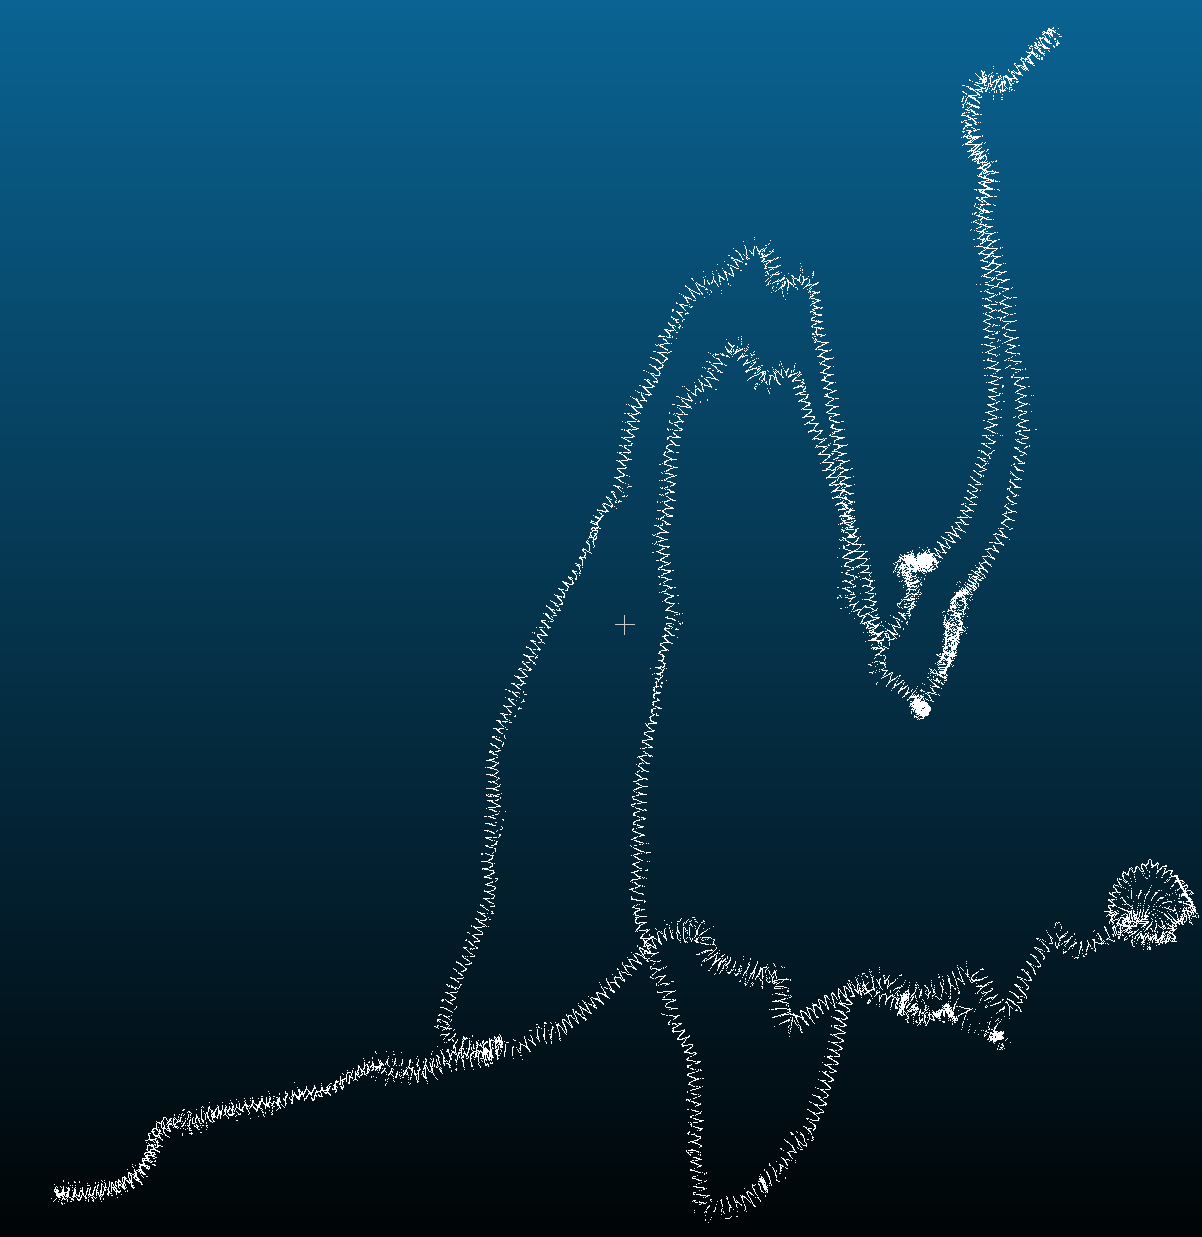
\includegraphics[width=0.9\linewidth, height=9cm, keepaspectratio]{figures/initial_point_cloud.png}
  \caption{Initial point cloud of the conduit obtained from the vertical sonar \citep{margaritis2025internship}.}
  \label{fig:bg_pointcloud}
\end{figure}

% ------------------------------------------------------------------------------
\subsection{The unused horizontal sonar}  % the gap this project addresses
\label{sec:bg_gap}                        % \secref{sec:bg_gap}

The point cloud of \citet{margaritis2025internship}, and everything built on it, uses only the
echoes of the vertical sonar. Each vertical scan describes one cross-section of the conduit, so
the map is a sequence of slices whose spacing along the conduit depends entirely on the estimated
trajectory. The horizontal sonar, recorded during the same dive, sees the walls along the
direction of travel and could provide extra information about the conduit geometry, but it was not used in that work.
(Figure~\ref{fig:bg_scanplanes}).

Exploiting it is, however, not trivial:
\begin{itemize}                          % why the horizontal sonar is hard to use
  \item \textbf{Elevation ambiguity:} with a beam 25$^\circ$ high, an echo may come from anywhere
        within that vertical aperture, so the height of a detected point is uncertain.
  \item \textbf{Motion during a scan:} a 360$^\circ$ sweep takes several seconds, during which the
        vehicle moves and turns, so each ping must be placed with its own pose.
  \item \textbf{Fusion of perpendicular scans:} the two sonars observe different planes, at
        different rates and with different noise, and must be expressed consistently in a single
        frame and point cloud.
\end{itemize}
The aim of this project is to process the horizontal sonar data and merge them with the vertical
sonar data into one consistent point cloud (\secref{sec:msis_merging}).

\begin{figure}[!htbp]                    % geometry of the two scanning planes
  \centering
  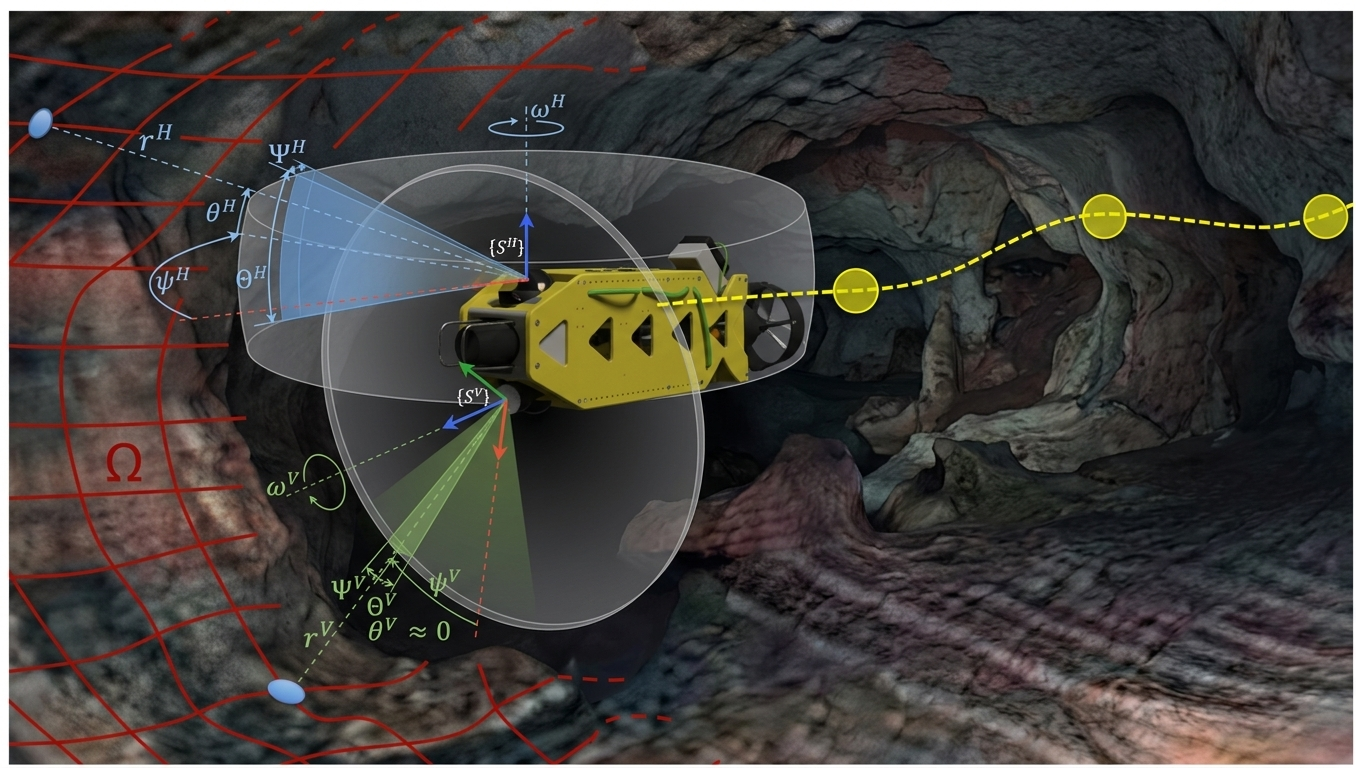
\includegraphics[width=0.9\linewidth, height=9cm, keepaspectratio]{figures/scanning_planes.jpeg}
  \caption{Scanning planes of the two MSIS on the NavScoot~2.}
  \label{fig:bg_scanplanes}
\end{figure}
